\chapter{Z Tanım Bölgesinde Luenberger Gözleyicisi}
Durum uzay modeli
\begin{equation}
    x(k)=A x(k-1)+Bu(k-1),\quad y(k-1)=C x(k-1)
\end{equation}
olmak üzere \textbf{Luenberger Gözleyicisi}
\begin{equation}
    \hat{x}(k)=A \hat{x}(k-1)+Bu(k-1)+L(y(k-1)-\hat{y}(k-1)),\quad \hat{y}(k-1)=C \hat{x}(k-1)
\end{equation}
olarak tanımlanmaktadır. Burada sistem modelinin bir benzeri kullanılmaktadır, fakat ek bir terim olarak sistem çıkışı ve gözleyici çıkışı farkının $L$ terimi ile çarpımı gözleyici durumlarına etki etmektedir. Bu etkinin seçilmesine gözleyici tasarımı denmektedir. Gözleyicinin amacı sistem durumlarını hesaplamaktır. Bu sebeple sistem durumları ve gözleyici durumları arasındaki fark, veya hata, $e(k)$ olmak üzere
\begin{equation}
    e(k)=x(k)-\hat{x}(k)
\end{equation}
olarak tanımlanır. Hatanın değişimi ise $\Delta e(k)$ olmak üzere,
\begin{equation}
\begin{split}
    \Delta e(k)&=\Delta (x(k)-\hat{x}(k))\\
    &=\Delta x(k)-\Delta\hat{x}(k)\\
    &=\frac{x(k)-x(k-1)}{T}-\frac{\hat{x}(k)-\hat{x}(k-1)}{T}\\
    &=\frac{A x(k-1)-x(k-1)-A\hat{x}(k-1)-L(y(k-1)-\hat{y}(k-1))+\hat{x}(k-1)}{T}\\
    &=\frac{A e(k-1)-e(k-1)-LC(x(k-1)-\hat{x}(k-1))}{T}\\
    &=\frac{A e(k-1)-e(k-1)-LCe(k-1)}{T}\\
    e(k)-e(k-1)&=(A-LC-I)e(k-1)\\
    e(k)&=(A-LC)e(k-1)
\end{split}
\end{equation}
elde edilir. Elde edilen sistemin kararlı kılınması durumunda 
\begin{equation}
\begin{split}
    e(k)&\rightarrow 0\\
    x(k)-\hat{x}(k)&\rightarrow 0\\
    x(k)&\rightarrow \hat{x}(k)
\end{split}
\end{equation}
olacağından, gözleyici çalışacaktır. Bunun için,
\begin{equation}
    p_c(s)=det(sI-(A-LC))
\end{equation}
ile elde edilen polinomun kutuplarının kararlı olacak şekilde seçilmesi gerekmektedir. Gözleyici katsayısı $L$ 
\begin{equation}
    L=p_d(A)\begin{bmatrix}C\\ CA\\ \vdots\\ CA^{n-1}\end{bmatrix}^{-1}\begin{bmatrix}0\\ 0\\ \vdots\\ 0\\ 1\end{bmatrix}
\end{equation}
ile seçilebilmektedir. Örnek olarak
\begin{equation}
    \begin{split}
\begin{bmatrix}
    x_1[k]\\
    x_2[k]
\end{bmatrix}&=
\begin{bmatrix}
    1& 0.1\\
    -0.1& 0.95
\end{bmatrix}\begin{bmatrix}
    x_1[k-1]\\
    x_2[k-1]
\end{bmatrix}+\begin{bmatrix}
    0\\
    0.1
\end{bmatrix}u[k-1]\\
y[k-1]&=\begin{bmatrix}
    1&0 
\end{bmatrix}\begin{bmatrix}
    x_1[k-1]\\
    x_2[k-1]
\end{bmatrix}\\
\end{split}
\end{equation}
ile verilen sistem için gözleyici katsayısı
\begin{equation}
\begin{split}
    L&=p_d(A)\begin{bmatrix}C\\ CA\\ \vdots\\ CA^{n-1}\end{bmatrix}^{-1}\begin{bmatrix}0\\ 0\\ \vdots\\ 0\\ 1\end{bmatrix}\\
    &=\begin{bmatrix} 0.8&0.1750\\-0.175&0.7125\end{bmatrix}
    \begin{bmatrix} 1&0\\1&0.1\end{bmatrix}^{-1}\begin{bmatrix}0\\ 1\end{bmatrix}\\
    &=\begin{bmatrix}1.75\\7.125\end{bmatrix}
\end{split}
\end{equation}
olarak hesaplamaktır. Elde edilen Luenberger gözleyicisi Şekil~\ref{fig:lec13_model1} ile gösterilmektedir.

\begin{figure}[!htb]
    \centering
    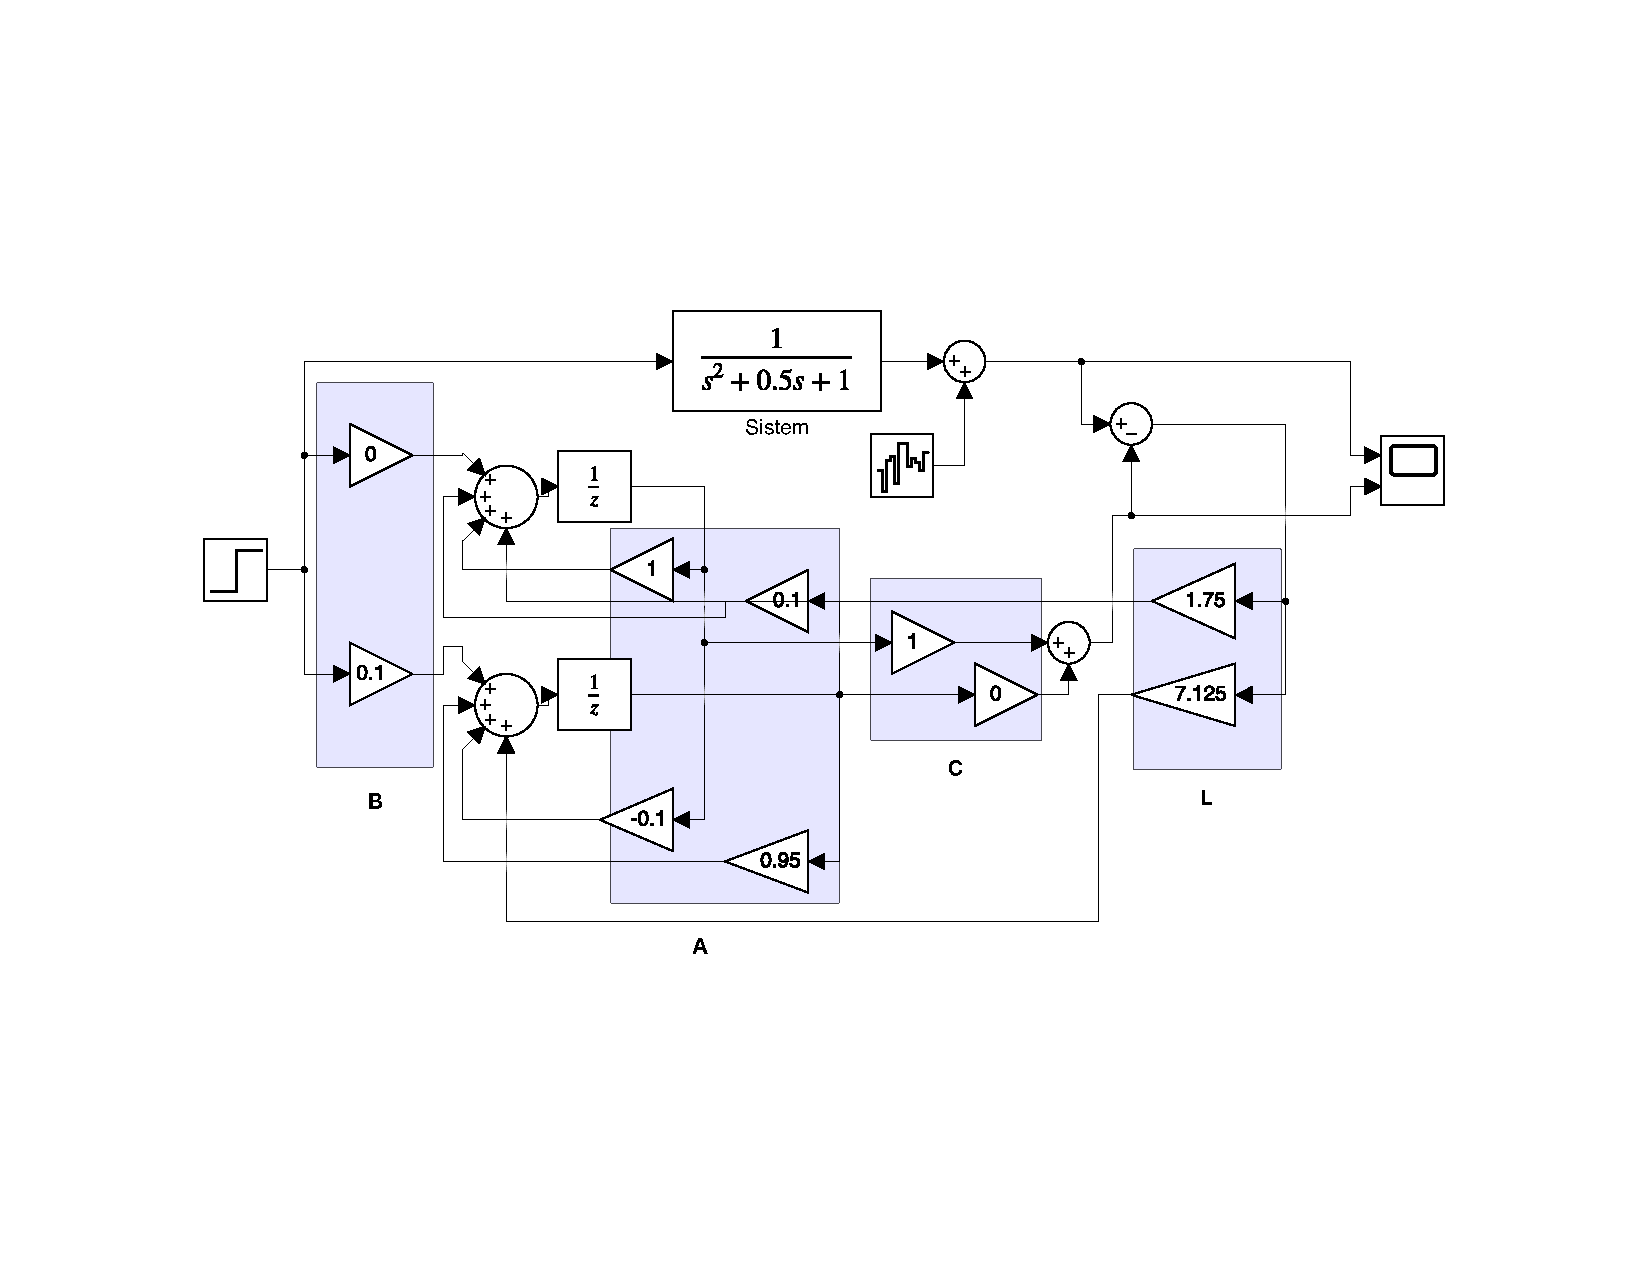
\includegraphics[width=\textwidth]{img/lec13_model1}
    \caption{Yay-kütle-damper sistemine ait gözleyici}
    \label{fig:lec13_model1}
\end{figure}

\begin{figure}[!htb]
    \centering
    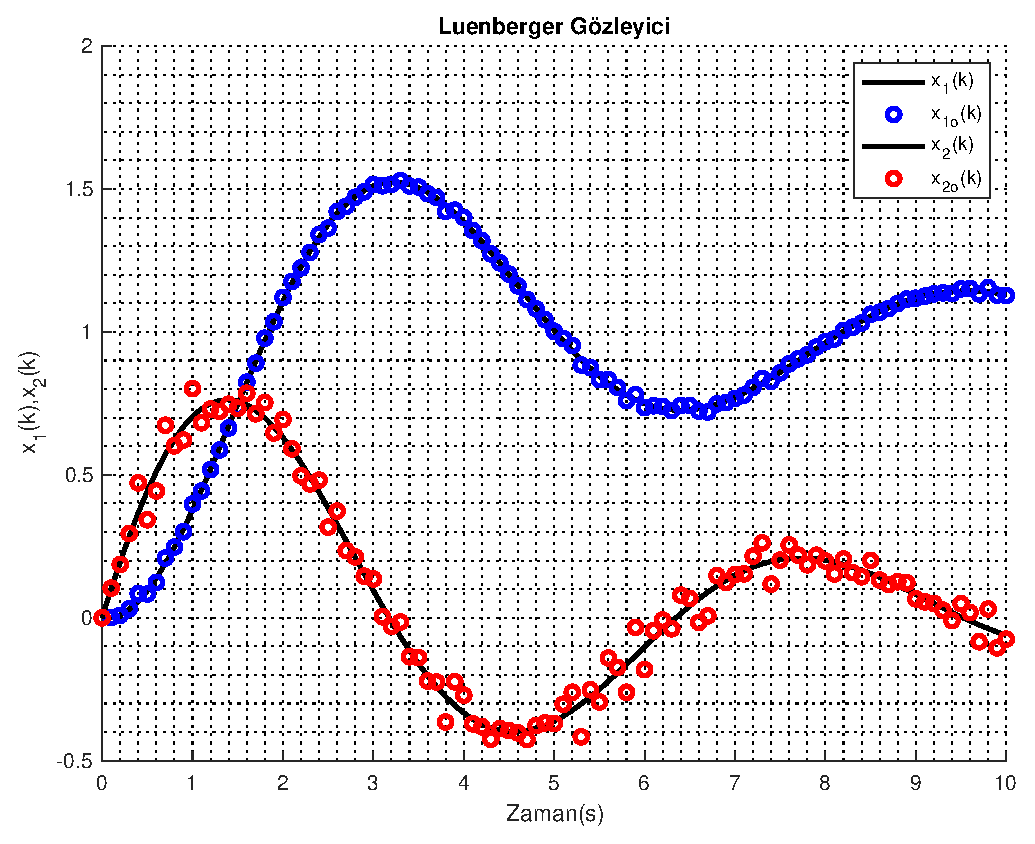
\includegraphics[width=0.75\textwidth]{img/lec13_plot1}
    \caption{Yay-kütle-damper sistemine ait gözleyici yanıtı}
    \label{fig:lec13_plot1}
\end{figure}